
\subsection{Datasets}
We used Europarl dataset and the data was numberized after tokenizing, splitting, and excluding xml markups. The first $10K$ sentences were used as the test data, and the last 80\% as the training data (See Table~\ref{fig:data}).

\begin{table}
\resizebox{1\columnwidth}{!}{
\begin{tabular}{ll|cc|c}
Language&&Size (MB)&Tokens (M)& Sentences (K)\\
\toprule 
Bulgarian&BG&36.11&8.53&329\\
Czech&CS&53.48&12.25&535\\
German&DE&171.80&44.07&1785 \\
English&EN&179.15&49.32&1815\\
Finnish&FI&145.32&32.85&1737\\
French&FR&197.68&53.82&1792\\
Hungarian&HU&52.53&12.02&527\\
Italian&IT&186.67&48.08&1703\\
Portuguese&PT&187.20&49.03&1737\\
\end{tabular}}
\caption{Tokens and sentence counts refer to the training partition. \trevor{Move to \supp}}\label{fig:data}
\end{table}
Figure~\ref{fig:data} is showing XXX.
\begin{figure}
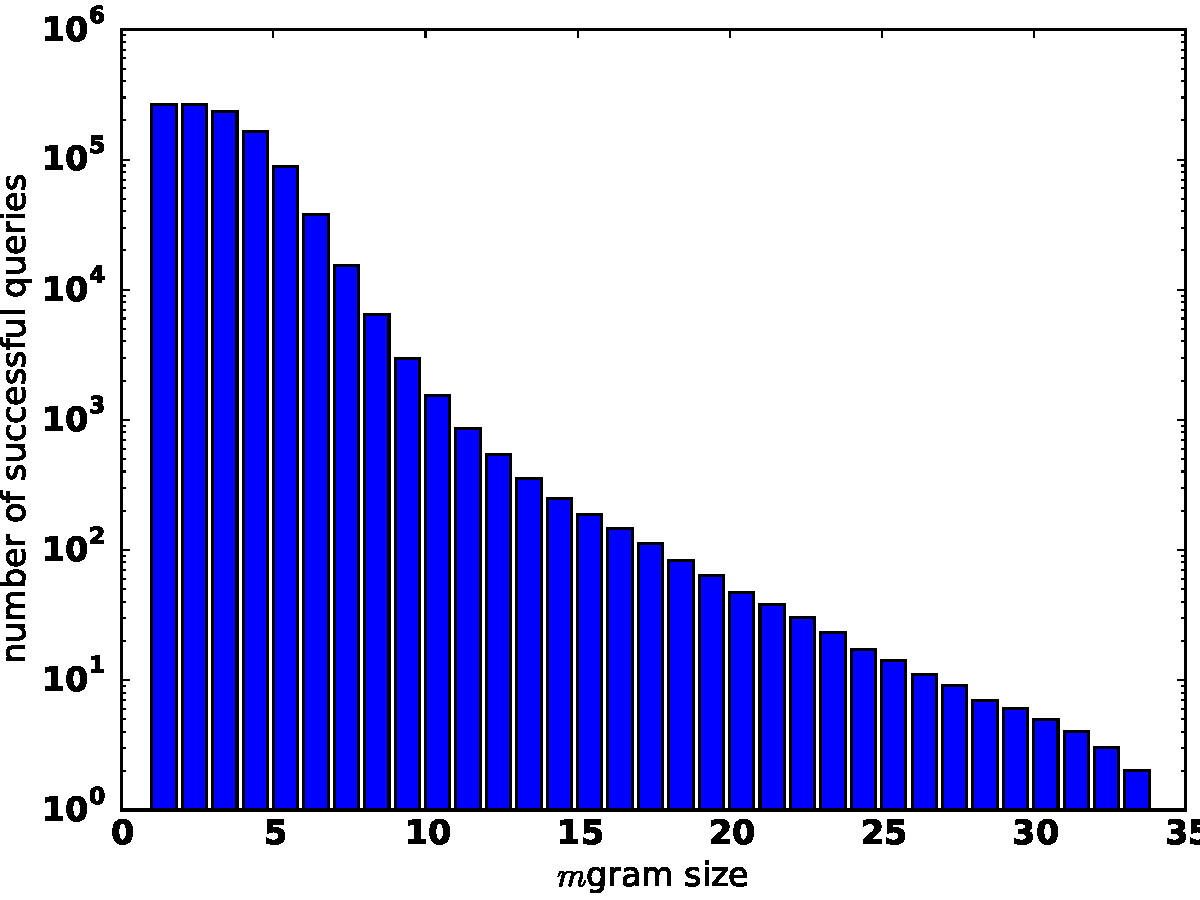
\includegraphics[width=\columnwidth]{figures/german_pattern_size.pdf}
\caption{Number of successful queries across different pattern sizes from KN computation over the German test set, with unbounded $m$.}
\end{figure}\label{fig:germanpattern}

\subsection{Perplexity Evaluation}
We evaluated the perplexity across different languages and using different order $m$-grams varying from $2$ to $\infty=99999$. While matching SRILM in perplexity we compared our time and memory usage during the training and query time with SRILM default (optimized for time), and compact(optimized for space). Figure~\ref{figure:pplx} shows the gain in perplexity with respect to $m$. 
\begin{figure}
% Created by tikzDevice version 0.8.1 on 2015-05-31 13:53:07
% !TEX encoding = UTF-8 Unicode
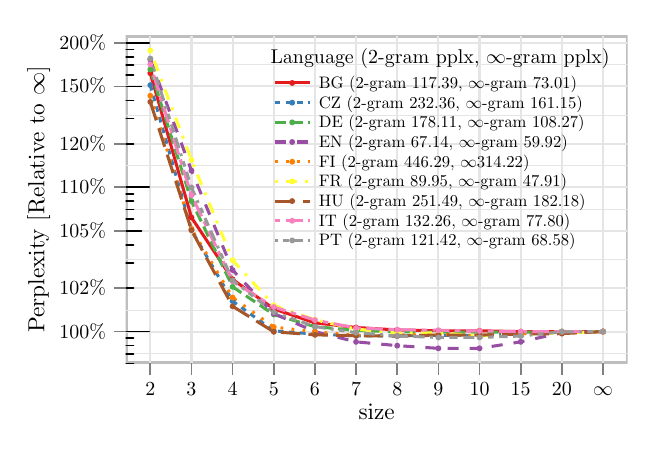
\begin{tikzpicture}[x=1pt,y=1pt]
\definecolor{fillColor}{RGB}{255,255,255}
\path[use as bounding box,fill=fillColor,fill opacity=0.00] (0,0) rectangle (216.81,144.54);
\begin{scope}
\path[clip] (  0.00,  0.00) rectangle (216.81,144.54);
\definecolor{fillColor}{RGB}{255,255,255}

\path[fill=fillColor] (  0.00,  0.00) rectangle (216.81,144.54);
\end{scope}
\begin{scope}
\path[clip] ( 35.40, 23.29) rectangle (216.81,141.69);
\definecolor{drawColor}{RGB}{190,190,190}

\path[draw=drawColor,line width= 1.5pt,line join=round,line cap=round] ( 35.40, 23.29) rectangle (216.81,141.69);
\definecolor{drawColor}{gray}{0.90}

\path[draw=drawColor,line width= 0.3pt,line join=round] ( 35.40, 26.85) --
	(216.81, 26.85);

\path[draw=drawColor,line width= 0.3pt,line join=round] ( 35.40, 42.55) --
	(216.81, 42.55);

\path[draw=drawColor,line width= 0.3pt,line join=round] ( 35.40, 60.78) --
	(216.81, 60.78);

\path[draw=drawColor,line width= 0.3pt,line join=round] ( 35.40, 79.01) --
	(216.81, 79.01);

\path[draw=drawColor,line width= 0.3pt,line join=round] ( 35.40, 94.71) --
	(216.81, 94.71);

\path[draw=drawColor,line width= 0.3pt,line join=round] ( 35.40,112.94) --
	(216.81,112.94);

\path[draw=drawColor,line width= 0.3pt,line join=round] ( 35.40,131.17) --
	(216.81,131.17);

\path[draw=drawColor,line width= 0.8pt,line join=round] ( 35.40, 34.70) --
	(216.81, 34.70);

\path[draw=drawColor,line width= 0.8pt,line join=round] ( 35.40, 50.40) --
	(216.81, 50.40);

\path[draw=drawColor,line width= 0.8pt,line join=round] ( 35.40, 71.16) --
	(216.81, 71.16);

\path[draw=drawColor,line width= 0.8pt,line join=round] ( 35.40, 86.86) --
	(216.81, 86.86);

\path[draw=drawColor,line width= 0.8pt,line join=round] ( 35.40,102.56) --
	(216.81,102.56);

\path[draw=drawColor,line width= 0.8pt,line join=round] ( 35.40,123.32) --
	(216.81,123.32);

\path[draw=drawColor,line width= 0.8pt,line join=round] ( 35.40,139.02) --
	(216.81,139.02);

\path[draw=drawColor,line width= 0.8pt,line join=round] ( 44.32, 23.29) --
	( 44.32,141.69);

\path[draw=drawColor,line width= 0.8pt,line join=round] ( 59.19, 23.29) --
	( 59.19,141.69);

\path[draw=drawColor,line width= 0.8pt,line join=round] ( 74.06, 23.29) --
	( 74.06,141.69);

\path[draw=drawColor,line width= 0.8pt,line join=round] ( 88.93, 23.29) --
	( 88.93,141.69);

\path[draw=drawColor,line width= 0.8pt,line join=round] (103.80, 23.29) --
	(103.80,141.69);

\path[draw=drawColor,line width= 0.8pt,line join=round] (118.67, 23.29) --
	(118.67,141.69);

\path[draw=drawColor,line width= 0.8pt,line join=round] (133.54, 23.29) --
	(133.54,141.69);

\path[draw=drawColor,line width= 0.8pt,line join=round] (148.41, 23.29) --
	(148.41,141.69);

\path[draw=drawColor,line width= 0.8pt,line join=round] (163.28, 23.29) --
	(163.28,141.69);

\path[draw=drawColor,line width= 0.8pt,line join=round] (178.15, 23.29) --
	(178.15,141.69);

\path[draw=drawColor,line width= 0.8pt,line join=round] (193.02, 23.29) --
	(193.02,141.69);

\path[draw=drawColor,line width= 0.8pt,line join=round] (207.89, 23.29) --
	(207.89,141.69);
\definecolor{drawColor}{RGB}{228,26,28}

\path[draw=drawColor,line width= 1.1pt,line join=round] ( 44.32,128.11) --
	( 59.19, 75.95) --
	( 74.06, 53.58) --
	( 88.93, 42.93) --
	(103.80, 37.88) --
	(118.67, 36.20) --
	(133.54, 35.31) --
	(148.41, 35.01) --
	(163.28, 35.01) --
	(178.15, 34.70) --
	(193.02, 34.70) --
	(207.89, 34.70);
\definecolor{drawColor}{RGB}{55,126,184}

\path[draw=drawColor,line width= 1.1pt,dash pattern=on 2pt off 2pt ,line join=round] ( 44.32,123.78) --
	( 59.19, 71.41) --
	( 74.06, 45.72) --
	( 88.93, 34.99) --
	(103.80, 33.81) --
	(118.67, 33.19) --
	(133.54, 33.19) --
	(148.41, 33.34) --
	(163.28, 33.34) --
	(178.15, 34.41) --
	(193.02, 34.55) --
	(207.89, 34.70);
\definecolor{drawColor}{RGB}{77,175,74}

\path[draw=drawColor,line width= 1.1pt,dash pattern=on 4pt off 2pt ,line join=round] ( 44.32,129.43) --
	( 59.19, 81.86) --
	( 74.06, 50.89) --
	( 88.93, 40.89) --
	(103.80, 36.51) --
	(118.67, 35.12) --
	(133.54, 34.70) --
	(148.41, 34.49) --
	(163.28, 34.49) --
	(178.15, 34.49) --
	(193.02, 34.70) --
	(207.89, 34.70);
\definecolor{drawColor}{RGB}{152,78,163}

\path[draw=drawColor,line width= 1.1pt,dash pattern=on 4pt off 4pt ,line join=round] ( 44.32,132.99) --
	( 59.19, 92.89) --
	( 74.06, 56.94) --
	( 88.93, 41.23) --
	(103.80, 34.70) --
	(118.67, 31.01) --
	(133.54, 29.64) --
	(148.41, 28.67) --
	(163.28, 28.67) --
	(178.15, 31.01) --
	(193.02, 34.32) --
	(207.89, 34.70);
\definecolor{drawColor}{RGB}{255,127,0}

\path[draw=drawColor,line width= 1.1pt,dash pattern=on 1pt off 3pt ,line join=round] ( 44.32,119.92) --
	( 59.19, 71.83) --
	( 74.06, 47.02) --
	( 88.93, 36.37) --
	(103.80, 34.63) --
	(118.67, 33.44) --
	(133.54, 33.52) --
	(148.41, 33.67) --
	(163.28, 33.29) --
	(178.15, 33.97) --
	(193.02, 34.48) --
	(207.89, 34.70);
\definecolor{drawColor}{RGB}{255,255,51}

\path[draw=drawColor,line width= 1.1pt,dash pattern=on 1pt off 3pt on 4pt off 3pt ,line join=round] ( 44.32,136.31) --
	( 59.19, 96.73) --
	( 74.06, 60.54) --
	( 88.93, 44.21) --
	(103.80, 38.99) --
	(118.67, 35.63) --
	(133.54, 34.22) --
	(148.41, 34.22) --
	(163.28, 33.24) --
	(178.15, 33.74) --
	(193.02, 34.22) --
	(207.89, 34.70);
\definecolor{drawColor}{RGB}{166,86,40}

\path[draw=drawColor,line width= 1.1pt,dash pattern=on 7pt off 3pt ,line join=round] ( 44.32,117.71) --
	( 59.19, 71.37) --
	( 74.06, 43.85) --
	( 88.93, 34.64) --
	(103.80, 33.55) --
	(118.67, 33.23) --
	(133.54, 33.12) --
	(148.41, 33.49) --
	(163.28, 33.45) --
	(178.15, 33.81) --
	(193.02, 33.99) --
	(207.89, 34.70);
\definecolor{drawColor}{RGB}{247,129,191}

\path[draw=drawColor,line width= 1.1pt,dash pattern=on 2pt off 2pt on 6pt off 2pt ,line join=round] ( 44.32,131.26) --
	( 59.19, 84.00) --
	( 74.06, 52.90) --
	( 88.93, 43.58) --
	(103.80, 38.87) --
	(118.67, 36.02) --
	(133.54, 35.40) --
	(148.41, 35.21) --
	(163.28, 34.95) --
	(178.15, 34.72) --
	(193.02, 34.69) --
	(207.89, 34.70);
\definecolor{drawColor}{gray}{0.60}

\path[draw=drawColor,line width= 1.1pt,dash pattern=on 1pt off 2pt on 2pt off 2pt on 3pt off 2pt on 4pt off 2pt ,line join=round] ( 44.32,133.40) --
	( 59.19, 86.79) --
	( 74.06, 53.23) --
	( 88.93, 41.73) --
	(103.80, 36.54) --
	(118.67, 34.31) --
	(133.54, 33.17) --
	(148.41, 32.59) --
	(163.28, 32.62) --
	(178.15, 33.11) --
	(193.02, 34.63) --
	(207.89, 34.70);
\definecolor{fillColor}{RGB}{228,26,28}

\path[fill=fillColor] ( 44.32,128.11) circle (  1.07);

\path[fill=fillColor] ( 59.19, 75.95) circle (  1.07);

\path[fill=fillColor] ( 74.06, 53.58) circle (  1.07);

\path[fill=fillColor] ( 88.93, 42.93) circle (  1.07);

\path[fill=fillColor] (103.80, 37.88) circle (  1.07);

\path[fill=fillColor] (118.67, 36.20) circle (  1.07);

\path[fill=fillColor] (133.54, 35.31) circle (  1.07);

\path[fill=fillColor] (148.41, 35.01) circle (  1.07);

\path[fill=fillColor] (163.28, 35.01) circle (  1.07);

\path[fill=fillColor] (178.15, 34.70) circle (  1.07);

\path[fill=fillColor] (193.02, 34.70) circle (  1.07);

\path[fill=fillColor] (207.89, 34.70) circle (  1.07);
\definecolor{fillColor}{RGB}{55,126,184}

\path[fill=fillColor] ( 44.32,123.78) circle (  1.07);

\path[fill=fillColor] ( 59.19, 71.41) circle (  1.07);

\path[fill=fillColor] ( 74.06, 45.72) circle (  1.07);

\path[fill=fillColor] ( 88.93, 34.99) circle (  1.07);

\path[fill=fillColor] (103.80, 33.81) circle (  1.07);

\path[fill=fillColor] (118.67, 33.19) circle (  1.07);

\path[fill=fillColor] (133.54, 33.19) circle (  1.07);

\path[fill=fillColor] (148.41, 33.34) circle (  1.07);

\path[fill=fillColor] (163.28, 33.34) circle (  1.07);

\path[fill=fillColor] (178.15, 34.41) circle (  1.07);

\path[fill=fillColor] (193.02, 34.55) circle (  1.07);

\path[fill=fillColor] (207.89, 34.70) circle (  1.07);
\definecolor{fillColor}{RGB}{77,175,74}

\path[fill=fillColor] ( 44.32,129.43) circle (  1.07);

\path[fill=fillColor] ( 59.19, 81.86) circle (  1.07);

\path[fill=fillColor] ( 74.06, 50.89) circle (  1.07);

\path[fill=fillColor] ( 88.93, 40.89) circle (  1.07);

\path[fill=fillColor] (103.80, 36.51) circle (  1.07);

\path[fill=fillColor] (118.67, 35.12) circle (  1.07);

\path[fill=fillColor] (133.54, 34.70) circle (  1.07);

\path[fill=fillColor] (148.41, 34.49) circle (  1.07);

\path[fill=fillColor] (163.28, 34.49) circle (  1.07);

\path[fill=fillColor] (178.15, 34.49) circle (  1.07);

\path[fill=fillColor] (193.02, 34.70) circle (  1.07);

\path[fill=fillColor] (207.89, 34.70) circle (  1.07);
\definecolor{fillColor}{RGB}{152,78,163}

\path[fill=fillColor] ( 44.32,132.99) circle (  1.07);

\path[fill=fillColor] ( 59.19, 92.89) circle (  1.07);

\path[fill=fillColor] ( 74.06, 56.94) circle (  1.07);

\path[fill=fillColor] ( 88.93, 41.23) circle (  1.07);

\path[fill=fillColor] (103.80, 34.70) circle (  1.07);

\path[fill=fillColor] (118.67, 31.01) circle (  1.07);

\path[fill=fillColor] (133.54, 29.64) circle (  1.07);

\path[fill=fillColor] (148.41, 28.67) circle (  1.07);

\path[fill=fillColor] (163.28, 28.67) circle (  1.07);

\path[fill=fillColor] (178.15, 31.01) circle (  1.07);

\path[fill=fillColor] (193.02, 34.32) circle (  1.07);

\path[fill=fillColor] (207.89, 34.70) circle (  1.07);
\definecolor{fillColor}{RGB}{255,127,0}

\path[fill=fillColor] ( 44.32,119.92) circle (  1.07);

\path[fill=fillColor] ( 59.19, 71.83) circle (  1.07);

\path[fill=fillColor] ( 74.06, 47.02) circle (  1.07);

\path[fill=fillColor] ( 88.93, 36.37) circle (  1.07);

\path[fill=fillColor] (103.80, 34.63) circle (  1.07);

\path[fill=fillColor] (118.67, 33.44) circle (  1.07);

\path[fill=fillColor] (133.54, 33.52) circle (  1.07);

\path[fill=fillColor] (148.41, 33.67) circle (  1.07);

\path[fill=fillColor] (163.28, 33.29) circle (  1.07);

\path[fill=fillColor] (178.15, 33.97) circle (  1.07);

\path[fill=fillColor] (193.02, 34.48) circle (  1.07);

\path[fill=fillColor] (207.89, 34.70) circle (  1.07);
\definecolor{fillColor}{RGB}{255,255,51}

\path[fill=fillColor] ( 44.32,136.31) circle (  1.07);

\path[fill=fillColor] ( 59.19, 96.73) circle (  1.07);

\path[fill=fillColor] ( 74.06, 60.54) circle (  1.07);

\path[fill=fillColor] ( 88.93, 44.21) circle (  1.07);

\path[fill=fillColor] (103.80, 38.99) circle (  1.07);

\path[fill=fillColor] (118.67, 35.63) circle (  1.07);

\path[fill=fillColor] (133.54, 34.22) circle (  1.07);

\path[fill=fillColor] (148.41, 34.22) circle (  1.07);

\path[fill=fillColor] (163.28, 33.24) circle (  1.07);

\path[fill=fillColor] (178.15, 33.74) circle (  1.07);

\path[fill=fillColor] (193.02, 34.22) circle (  1.07);

\path[fill=fillColor] (207.89, 34.70) circle (  1.07);
\definecolor{fillColor}{RGB}{166,86,40}

\path[fill=fillColor] ( 44.32,117.71) circle (  1.07);

\path[fill=fillColor] ( 59.19, 71.37) circle (  1.07);

\path[fill=fillColor] ( 74.06, 43.85) circle (  1.07);

\path[fill=fillColor] ( 88.93, 34.64) circle (  1.07);

\path[fill=fillColor] (103.80, 33.55) circle (  1.07);

\path[fill=fillColor] (118.67, 33.23) circle (  1.07);

\path[fill=fillColor] (133.54, 33.12) circle (  1.07);

\path[fill=fillColor] (148.41, 33.49) circle (  1.07);

\path[fill=fillColor] (163.28, 33.45) circle (  1.07);

\path[fill=fillColor] (178.15, 33.81) circle (  1.07);

\path[fill=fillColor] (193.02, 33.99) circle (  1.07);

\path[fill=fillColor] (207.89, 34.70) circle (  1.07);
\definecolor{fillColor}{RGB}{247,129,191}

\path[fill=fillColor] ( 44.32,131.26) circle (  1.07);

\path[fill=fillColor] ( 59.19, 84.00) circle (  1.07);

\path[fill=fillColor] ( 74.06, 52.90) circle (  1.07);

\path[fill=fillColor] ( 88.93, 43.58) circle (  1.07);

\path[fill=fillColor] (103.80, 38.87) circle (  1.07);

\path[fill=fillColor] (118.67, 36.02) circle (  1.07);

\path[fill=fillColor] (133.54, 35.40) circle (  1.07);

\path[fill=fillColor] (148.41, 35.21) circle (  1.07);

\path[fill=fillColor] (163.28, 34.95) circle (  1.07);

\path[fill=fillColor] (178.15, 34.72) circle (  1.07);

\path[fill=fillColor] (193.02, 34.69) circle (  1.07);

\path[fill=fillColor] (207.89, 34.70) circle (  1.07);
\definecolor{fillColor}{gray}{0.60}

\path[fill=fillColor] ( 44.32,133.40) circle (  1.07);

\path[fill=fillColor] ( 59.19, 86.79) circle (  1.07);

\path[fill=fillColor] ( 74.06, 53.23) circle (  1.07);

\path[fill=fillColor] ( 88.93, 41.73) circle (  1.07);

\path[fill=fillColor] (103.80, 36.54) circle (  1.07);

\path[fill=fillColor] (118.67, 34.31) circle (  1.07);

\path[fill=fillColor] (133.54, 33.17) circle (  1.07);

\path[fill=fillColor] (148.41, 32.59) circle (  1.07);

\path[fill=fillColor] (163.28, 32.62) circle (  1.07);

\path[fill=fillColor] (178.15, 33.11) circle (  1.07);

\path[fill=fillColor] (193.02, 34.63) circle (  1.07);

\path[fill=fillColor] (207.89, 34.70) circle (  1.07);
\definecolor{drawColor}{RGB}{0,0,0}

\path[draw=drawColor,line width= 0.6pt,line join=round,line cap=round] ( 35.40,  7.43) -- ( 38.25,  7.43);

\path[draw=drawColor,line width= 0.6pt,line join=round,line cap=round] ( 35.40, 13.95) -- ( 38.25, 13.95);

\path[draw=drawColor,line width= 0.6pt,line join=round,line cap=round] ( 35.40, 19.00) -- ( 41.09, 19.00);

\path[draw=drawColor,line width= 0.6pt,line join=round,line cap=round] ( 35.40, 23.13) -- ( 38.25, 23.13);

\path[draw=drawColor,line width= 0.6pt,line join=round,line cap=round] ( 35.40, 26.62) -- ( 38.25, 26.62);

\path[draw=drawColor,line width= 0.6pt,line join=round,line cap=round] ( 35.40, 29.65) -- ( 38.25, 29.65);

\path[draw=drawColor,line width= 0.6pt,line join=round,line cap=round] ( 35.40, 32.31) -- ( 38.25, 32.31);

\path[draw=drawColor,line width= 0.6pt,line join=round,line cap=round] ( 35.40, 34.70) -- ( 43.94, 34.70);

\path[draw=drawColor,line width= 0.6pt,line join=round,line cap=round] ( 35.40, 50.40) -- ( 38.25, 50.40);

\path[draw=drawColor,line width= 0.6pt,line join=round,line cap=round] ( 35.40, 59.59) -- ( 38.25, 59.59);

\path[draw=drawColor,line width= 0.6pt,line join=round,line cap=round] ( 35.40, 66.10) -- ( 38.25, 66.10);

\path[draw=drawColor,line width= 0.6pt,line join=round,line cap=round] ( 35.40, 71.16) -- ( 41.09, 71.16);

\path[draw=drawColor,line width= 0.6pt,line join=round,line cap=round] ( 35.40, 75.29) -- ( 38.25, 75.29);

\path[draw=drawColor,line width= 0.6pt,line join=round,line cap=round] ( 35.40, 78.78) -- ( 38.25, 78.78);

\path[draw=drawColor,line width= 0.6pt,line join=round,line cap=round] ( 35.40, 81.80) -- ( 38.25, 81.80);

\path[draw=drawColor,line width= 0.6pt,line join=round,line cap=round] ( 35.40, 84.47) -- ( 38.25, 84.47);

\path[draw=drawColor,line width= 0.6pt,line join=round,line cap=round] ( 35.40, 86.86) -- ( 43.94, 86.86);

\path[draw=drawColor,line width= 0.6pt,line join=round,line cap=round] ( 35.40,102.56) -- ( 38.25,102.56);

\path[draw=drawColor,line width= 0.6pt,line join=round,line cap=round] ( 35.40,111.74) -- ( 38.25,111.74);

\path[draw=drawColor,line width= 0.6pt,line join=round,line cap=round] ( 35.40,118.26) -- ( 38.25,118.26);

\path[draw=drawColor,line width= 0.6pt,line join=round,line cap=round] ( 35.40,123.32) -- ( 41.09,123.32);

\path[draw=drawColor,line width= 0.6pt,line join=round,line cap=round] ( 35.40,127.45) -- ( 38.25,127.45);

\path[draw=drawColor,line width= 0.6pt,line join=round,line cap=round] ( 35.40,130.94) -- ( 38.25,130.94);

\path[draw=drawColor,line width= 0.6pt,line join=round,line cap=round] ( 35.40,133.96) -- ( 38.25,133.96);

\path[draw=drawColor,line width= 0.6pt,line join=round,line cap=round] ( 35.40,136.63) -- ( 38.25,136.63);

\path[draw=drawColor,line width= 0.6pt,line join=round,line cap=round] ( 35.40,139.02) -- ( 43.94,139.02);
\end{scope}
\begin{scope}
\path[clip] (  0.00,  0.00) rectangle (216.81,144.54);
\definecolor{drawColor}{RGB}{0,0,0}

\node[text=drawColor,anchor=base east,inner sep=0pt, outer sep=0pt, scale=  0.72] at ( 28.29, 32.36) {100\%};

\node[text=drawColor,anchor=base east,inner sep=0pt, outer sep=0pt, scale=  0.72] at ( 28.29, 48.06) {102\%};

\node[text=drawColor,anchor=base east,inner sep=0pt, outer sep=0pt, scale=  0.72] at ( 28.29, 68.81) {105\%};

\node[text=drawColor,anchor=base east,inner sep=0pt, outer sep=0pt, scale=  0.72] at ( 28.29, 84.52) {110\%};

\node[text=drawColor,anchor=base east,inner sep=0pt, outer sep=0pt, scale=  0.72] at ( 28.29,100.22) {120\%};

\node[text=drawColor,anchor=base east,inner sep=0pt, outer sep=0pt, scale=  0.72] at ( 28.29,120.97) {150\%};

\node[text=drawColor,anchor=base east,inner sep=0pt, outer sep=0pt, scale=  0.72] at ( 28.29,136.67) {200\%};
\end{scope}
\begin{scope}
\path[clip] (  0.00,  0.00) rectangle (216.81,144.54);
\definecolor{drawColor}{gray}{0.50}

\path[draw=drawColor,line width= 0.6pt,line join=round] ( 31.13, 34.70) --
	( 35.40, 34.70);

\path[draw=drawColor,line width= 0.6pt,line join=round] ( 31.13, 50.40) --
	( 35.40, 50.40);

\path[draw=drawColor,line width= 0.6pt,line join=round] ( 31.13, 71.16) --
	( 35.40, 71.16);

\path[draw=drawColor,line width= 0.6pt,line join=round] ( 31.13, 86.86) --
	( 35.40, 86.86);

\path[draw=drawColor,line width= 0.6pt,line join=round] ( 31.13,102.56) --
	( 35.40,102.56);

\path[draw=drawColor,line width= 0.6pt,line join=round] ( 31.13,123.32) --
	( 35.40,123.32);

\path[draw=drawColor,line width= 0.6pt,line join=round] ( 31.13,139.02) --
	( 35.40,139.02);
\end{scope}
\begin{scope}
\path[clip] (  0.00,  0.00) rectangle (216.81,144.54);
\definecolor{drawColor}{gray}{0.50}

\path[draw=drawColor,line width= 0.6pt,line join=round] ( 44.32, 19.02) --
	( 44.32, 23.29);

\path[draw=drawColor,line width= 0.6pt,line join=round] ( 59.19, 19.02) --
	( 59.19, 23.29);

\path[draw=drawColor,line width= 0.6pt,line join=round] ( 74.06, 19.02) --
	( 74.06, 23.29);

\path[draw=drawColor,line width= 0.6pt,line join=round] ( 88.93, 19.02) --
	( 88.93, 23.29);

\path[draw=drawColor,line width= 0.6pt,line join=round] (103.80, 19.02) --
	(103.80, 23.29);

\path[draw=drawColor,line width= 0.6pt,line join=round] (118.67, 19.02) --
	(118.67, 23.29);

\path[draw=drawColor,line width= 0.6pt,line join=round] (133.54, 19.02) --
	(133.54, 23.29);

\path[draw=drawColor,line width= 0.6pt,line join=round] (148.41, 19.02) --
	(148.41, 23.29);

\path[draw=drawColor,line width= 0.6pt,line join=round] (163.28, 19.02) --
	(163.28, 23.29);

\path[draw=drawColor,line width= 0.6pt,line join=round] (178.15, 19.02) --
	(178.15, 23.29);

\path[draw=drawColor,line width= 0.6pt,line join=round] (193.02, 19.02) --
	(193.02, 23.29);

\path[draw=drawColor,line width= 0.6pt,line join=round] (207.89, 19.02) --
	(207.89, 23.29);
\end{scope}
\begin{scope}
\path[clip] (  0.00,  0.00) rectangle (216.81,144.54);
\definecolor{drawColor}{RGB}{0,0,0}

\node[text=drawColor,anchor=base,inner sep=0pt, outer sep=0pt, scale=  0.72] at ( 44.32, 11.49) {2};

\node[text=drawColor,anchor=base,inner sep=0pt, outer sep=0pt, scale=  0.72] at ( 59.19, 11.49) {3};

\node[text=drawColor,anchor=base,inner sep=0pt, outer sep=0pt, scale=  0.72] at ( 74.06, 11.49) {4};

\node[text=drawColor,anchor=base,inner sep=0pt, outer sep=0pt, scale=  0.72] at ( 88.93, 11.49) {5};

\node[text=drawColor,anchor=base,inner sep=0pt, outer sep=0pt, scale=  0.72] at (103.80, 11.49) {6};

\node[text=drawColor,anchor=base,inner sep=0pt, outer sep=0pt, scale=  0.72] at (118.67, 11.49) {7};

\node[text=drawColor,anchor=base,inner sep=0pt, outer sep=0pt, scale=  0.72] at (133.54, 11.49) {8};

\node[text=drawColor,anchor=base,inner sep=0pt, outer sep=0pt, scale=  0.72] at (148.41, 11.49) {9};

\node[text=drawColor,anchor=base,inner sep=0pt, outer sep=0pt, scale=  0.72] at (163.28, 11.49) {10};

\node[text=drawColor,anchor=base,inner sep=0pt, outer sep=0pt, scale=  0.72] at (178.15, 11.49) {15};

\node[text=drawColor,anchor=base,inner sep=0pt, outer sep=0pt, scale=  0.72] at (193.02, 11.49) {20};

\node[text=drawColor,anchor=base,inner sep=0pt, outer sep=0pt, scale=  0.72] at (207.89, 11.49) {$\infty$};
\end{scope}
\begin{scope}
\path[clip] (  0.00,  0.00) rectangle (216.81,144.54);
\definecolor{drawColor}{RGB}{0,0,0}

\node[text=drawColor,anchor=base,inner sep=0pt, outer sep=0pt, scale=  0.84] at (126.11,  3.01) {\ngram size};
\end{scope}
\begin{scope}
\path[clip] (  0.00,  0.00) rectangle (216.81,144.54);
\definecolor{drawColor}{RGB}{0,0,0}

\node[text=drawColor,rotate= 90.00,anchor=base,inner sep=0pt, outer sep=0pt, scale=  0.84] at (  6.07, 82.49) {Perplexity [Relative to $\infty$]};
\end{scope}
\begin{scope}
\path[clip] (  0.00,  0.00) rectangle (216.81,144.54);
\definecolor{drawColor}{RGB}{0,0,0}

\node[text=drawColor,anchor=base west,inner sep=0pt, outer sep=0pt, scale=  0.72] at ( 87.76,131.73) {Language ($2$-gram pplx, $\infty$-gram pplx)};
\end{scope}
\begin{scope}
\path[clip] (  0.00,  0.00) rectangle (216.81,144.54);
\definecolor{drawColor}{RGB}{228,26,28}

\path[draw=drawColor,line width= 1.1pt,line join=round] ( 89.32,124.56) -- (101.84,124.56);
\end{scope}
\begin{scope}
\path[clip] (  0.00,  0.00) rectangle (216.81,144.54);
\definecolor{fillColor}{RGB}{228,26,28}

\path[fill=fillColor] ( 95.58,124.56) circle (  1.07);
\end{scope}
\begin{scope}
\path[clip] (  0.00,  0.00) rectangle (216.81,144.54);
\definecolor{drawColor}{RGB}{55,126,184}

\path[draw=drawColor,line width= 1.1pt,dash pattern=on 2pt off 2pt ,line join=round] ( 89.32,117.44) -- (101.84,117.44);
\end{scope}
\begin{scope}
\path[clip] (  0.00,  0.00) rectangle (216.81,144.54);
\definecolor{fillColor}{RGB}{55,126,184}

\path[fill=fillColor] ( 95.58,117.44) circle (  1.07);
\end{scope}
\begin{scope}
\path[clip] (  0.00,  0.00) rectangle (216.81,144.54);
\definecolor{drawColor}{RGB}{77,175,74}

\path[draw=drawColor,line width= 1.1pt,dash pattern=on 4pt off 2pt ,line join=round] ( 89.32,110.33) -- (101.84,110.33);
\end{scope}
\begin{scope}
\path[clip] (  0.00,  0.00) rectangle (216.81,144.54);
\definecolor{fillColor}{RGB}{77,175,74}

\path[fill=fillColor] ( 95.58,110.33) circle (  1.07);
\end{scope}
\begin{scope}
\path[clip] (  0.00,  0.00) rectangle (216.81,144.54);
\definecolor{drawColor}{RGB}{152,78,163}

\path[draw=drawColor,line width= 1.1pt,dash pattern=on 4pt off 4pt ,line join=round] ( 89.32,103.22) -- (101.84,103.22);
\end{scope}
\begin{scope}
\path[clip] (  0.00,  0.00) rectangle (216.81,144.54);
\definecolor{fillColor}{RGB}{152,78,163}

\path[fill=fillColor] ( 95.58,103.22) circle (  1.07);
\end{scope}
\begin{scope}
\path[clip] (  0.00,  0.00) rectangle (216.81,144.54);
\definecolor{drawColor}{RGB}{255,127,0}

\path[draw=drawColor,line width= 1.1pt,dash pattern=on 1pt off 3pt ,line join=round] ( 89.32, 96.10) -- (101.84, 96.10);
\end{scope}
\begin{scope}
\path[clip] (  0.00,  0.00) rectangle (216.81,144.54);
\definecolor{fillColor}{RGB}{255,127,0}

\path[fill=fillColor] ( 95.58, 96.10) circle (  1.07);
\end{scope}
\begin{scope}
\path[clip] (  0.00,  0.00) rectangle (216.81,144.54);
\definecolor{drawColor}{RGB}{255,255,51}

\path[draw=drawColor,line width= 1.1pt,dash pattern=on 1pt off 3pt on 4pt off 3pt ,line join=round] ( 89.32, 88.99) -- (101.84, 88.99);
\end{scope}
\begin{scope}
\path[clip] (  0.00,  0.00) rectangle (216.81,144.54);
\definecolor{fillColor}{RGB}{255,255,51}

\path[fill=fillColor] ( 95.58, 88.99) circle (  1.07);
\end{scope}
\begin{scope}
\path[clip] (  0.00,  0.00) rectangle (216.81,144.54);
\definecolor{drawColor}{RGB}{166,86,40}

\path[draw=drawColor,line width= 1.1pt,dash pattern=on 7pt off 3pt ,line join=round] ( 89.32, 81.88) -- (101.84, 81.88);
\end{scope}
\begin{scope}
\path[clip] (  0.00,  0.00) rectangle (216.81,144.54);
\definecolor{fillColor}{RGB}{166,86,40}

\path[fill=fillColor] ( 95.58, 81.88) circle (  1.07);
\end{scope}
\begin{scope}
\path[clip] (  0.00,  0.00) rectangle (216.81,144.54);
\definecolor{drawColor}{RGB}{247,129,191}

\path[draw=drawColor,line width= 1.1pt,dash pattern=on 2pt off 2pt on 6pt off 2pt ,line join=round] ( 89.32, 74.76) -- (101.84, 74.76);
\end{scope}
\begin{scope}
\path[clip] (  0.00,  0.00) rectangle (216.81,144.54);
\definecolor{fillColor}{RGB}{247,129,191}

\path[fill=fillColor] ( 95.58, 74.76) circle (  1.07);
\end{scope}
\begin{scope}
\path[clip] (  0.00,  0.00) rectangle (216.81,144.54);
\definecolor{drawColor}{gray}{0.60}

\path[draw=drawColor,line width= 1.1pt,dash pattern=on 1pt off 2pt on 2pt off 2pt on 3pt off 2pt on 4pt off 2pt ,line join=round] ( 89.32, 67.65) -- (101.84, 67.65);
\end{scope}
\begin{scope}
\path[clip] (  0.00,  0.00) rectangle (216.81,144.54);
\definecolor{fillColor}{gray}{0.60}

\path[fill=fillColor] ( 95.58, 67.65) circle (  1.07);
\end{scope}
\begin{scope}
\path[clip] (  0.00,  0.00) rectangle (216.81,144.54);
\definecolor{drawColor}{RGB}{0,0,0}

\node[text=drawColor,anchor=base west,inner sep=0pt, outer sep=0pt, scale=  0.60] at (105.22,122.60) {BG ($2$-gram $117.39$, $\infty$-gram $73.01$)};
\end{scope}
\begin{scope}
\path[clip] (  0.00,  0.00) rectangle (216.81,144.54);
\definecolor{drawColor}{RGB}{0,0,0}

\node[text=drawColor,anchor=base west,inner sep=0pt, outer sep=0pt, scale=  0.60] at (105.22,115.49) {CZ ($2$-gram $232.36$, $\infty$-gram $161.15$)};
\end{scope}
\begin{scope}
\path[clip] (  0.00,  0.00) rectangle (216.81,144.54);
\definecolor{drawColor}{RGB}{0,0,0}

\node[text=drawColor,anchor=base west,inner sep=0pt, outer sep=0pt, scale=  0.60] at (105.22,108.38) {DE ($2$-gram $178.11$, $\infty$-gram $108.27$)};
\end{scope}
\begin{scope}
\path[clip] (  0.00,  0.00) rectangle (216.81,144.54);
\definecolor{drawColor}{RGB}{0,0,0}

\node[text=drawColor,anchor=base west,inner sep=0pt, outer sep=0pt, scale=  0.60] at (105.22,101.26) {EN ($2$-gram $67.14$, $\infty$-gram $59.92$)};
\end{scope}
\begin{scope}
\path[clip] (  0.00,  0.00) rectangle (216.81,144.54);
\definecolor{drawColor}{RGB}{0,0,0}

\node[text=drawColor,anchor=base west,inner sep=0pt, outer sep=0pt, scale=  0.60] at (105.22, 94.15) {FI ($2$-gram $446.29$, $\infty 314.22$)};
\end{scope}
\begin{scope}
\path[clip] (  0.00,  0.00) rectangle (216.81,144.54);
\definecolor{drawColor}{RGB}{0,0,0}

\node[text=drawColor,anchor=base west,inner sep=0pt, outer sep=0pt, scale=  0.60] at (105.22, 87.04) {FR ($2$-gram $89.95$, $\infty$-gram $47.91$)};
\end{scope}
\begin{scope}
\path[clip] (  0.00,  0.00) rectangle (216.81,144.54);
\definecolor{drawColor}{RGB}{0,0,0}

\node[text=drawColor,anchor=base west,inner sep=0pt, outer sep=0pt, scale=  0.60] at (105.22, 79.92) {HU ($2$-gram $251.49$, $\infty$-gram $182.18$)};
\end{scope}
\begin{scope}
\path[clip] (  0.00,  0.00) rectangle (216.81,144.54);
\definecolor{drawColor}{RGB}{0,0,0}

\node[text=drawColor,anchor=base west,inner sep=0pt, outer sep=0pt, scale=  0.60] at (105.22, 72.81) {IT ($2$-gram $132.26$, $\infty$-gram $77.80$)};
\end{scope}
\begin{scope}
\path[clip] (  0.00,  0.00) rectangle (216.81,144.54);
\definecolor{drawColor}{RGB}{0,0,0}

\node[text=drawColor,anchor=base west,inner sep=0pt, outer sep=0pt, scale=  0.60] at (105.22, 65.70) {PT ($2$-gram $121.42$, $\infty$-gram $68.58$)};
\end{scope}
\end{tikzpicture}

\caption{All 8 languages pplx results with m=2..10,15,20,infinity(=99999).}
\end{figure}\label{figure:pplx}
We speculate that the drop in higher order perplexity gain is due using to Kneser-Ney discounting which is not designed for higher order $m$-gram language models and starts to heavily discount after $5-gram$. We leave further exploration of richer techniques such as Modified Kneser-Ney, or Sequence Memoizer to our future work. 
\subsection{Time-Memory}
Figure~\ref{figure:time-space} ($\log10-\log10$) compares our timing and memory usage with SRILM on German part of the Europarl dataset and highlights the merits of our method both in construction and query time. In construction time, while both of our approaches are independent of the order of $m$gram, our fixed construction time outperforms both SRILM methods in terms of memory for $m$grams of $5$ and higher orders. In terms of the timing, we outperform SRILM compact after bigram, and SRILM default for $m$grams of $3$ and higher orders.

In query time, our memory footprint is constant and much lower that SRILM compact, and default after $3$, and $2$ respectively. While in terms of timing, the single CST method is $300x$ slower compared to SRILM, but reduces the speed gap to $12x$.  

Another observation is the computational cost of computing $\nlplus{\Bigcdot w_{i-k+1}^{i-1} \Bigdot}$ when moving from $2$-gram, to $3$-gram which affects the timing. As mentioned earlier, this quantity is not required unless we move to $3$ or higher order $m$grams.

\begin{figure}
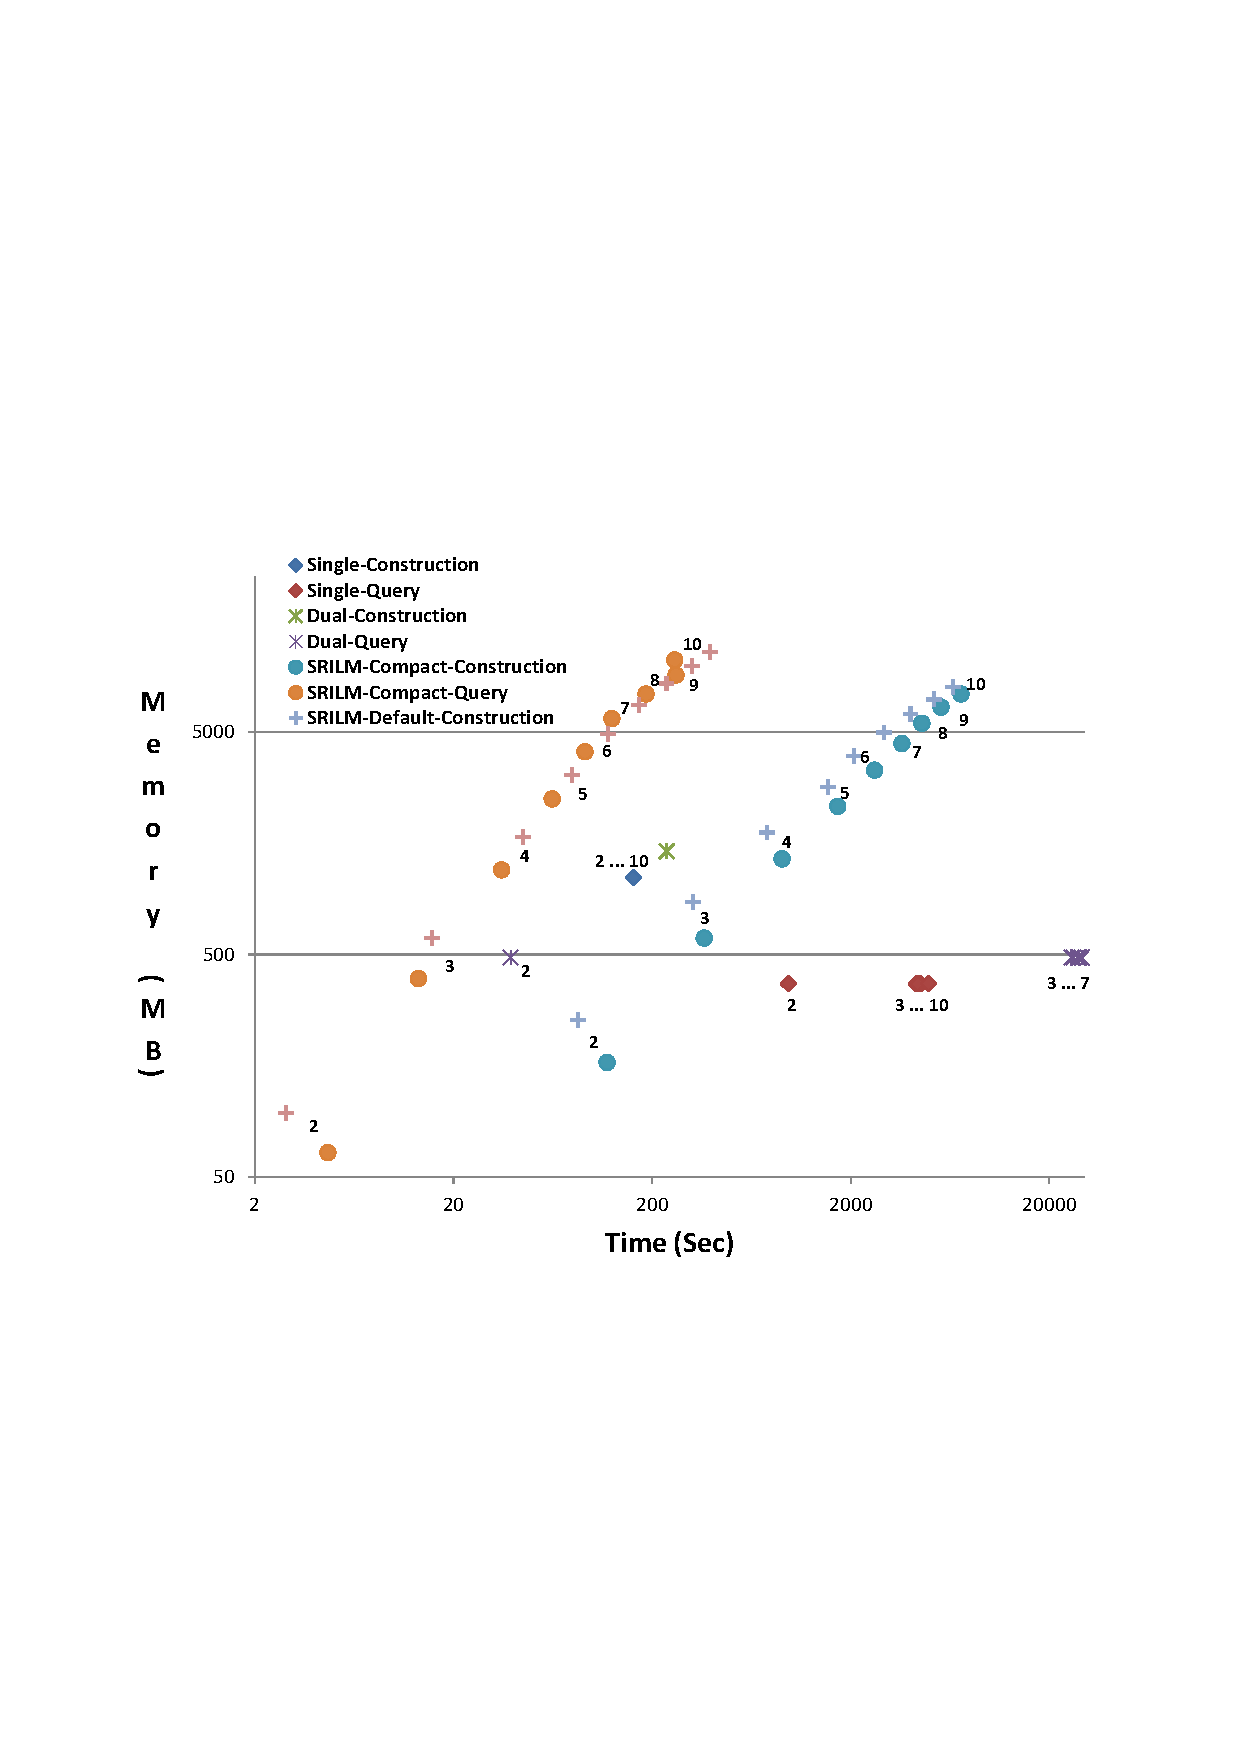
\includegraphics[width=\columnwidth]{figures/Time-Space.pdf}
\caption{On German, showing the size in MB (y axis) and time (x axis) for 4 methods: CST single, CST dual, SRILM, SRILM compact.}
\end{figure}\label{figure:time-space}
%\missingfigure[figwidth=\columnwidth]{Wikipedia pplx (right axis), and time (left axis) for the single CST on characters vs words as a function of \ngram size.}

%\missingfigure[figwidth=\columnwidth]{Wikipedia histogram over \ngram size, perhaps as a figure or table?}

%\missingfigure[figwidth=\columnwidth]{Wikipedia plot (stacked bar?) of time spent in each method (n1+ x 3; backward search etc) as a function of n.}






%%% Local Variables: 
%%% mode: latex
%%% TeX-master: "cstlm"
%%% End: 
